\documentclass[11pt,a4paper]{article}

\usepackage[a4paper]{geometry}
\geometry{hscale=0.85,vscale=0.85,centering}

\usepackage[utf8]{inputenc}
\usepackage{tikz}
\usetikzlibrary{positioning,chains,shapes}
\tikzset{
  boite/.style={
    rectangle,
    rounded corners,
    draw=black,very thick,
    text width=12em, 
    minimum height=3em, 
    text centered, 
    on chain},
  boiteif/.style={
    diamond,
    rounded corners,
    draw=black,very thick,
    text width=10em, 
    minimum height=3em, 
    text centered, 
    on chain},
  line/.style = {draw},
}
\begin{document}

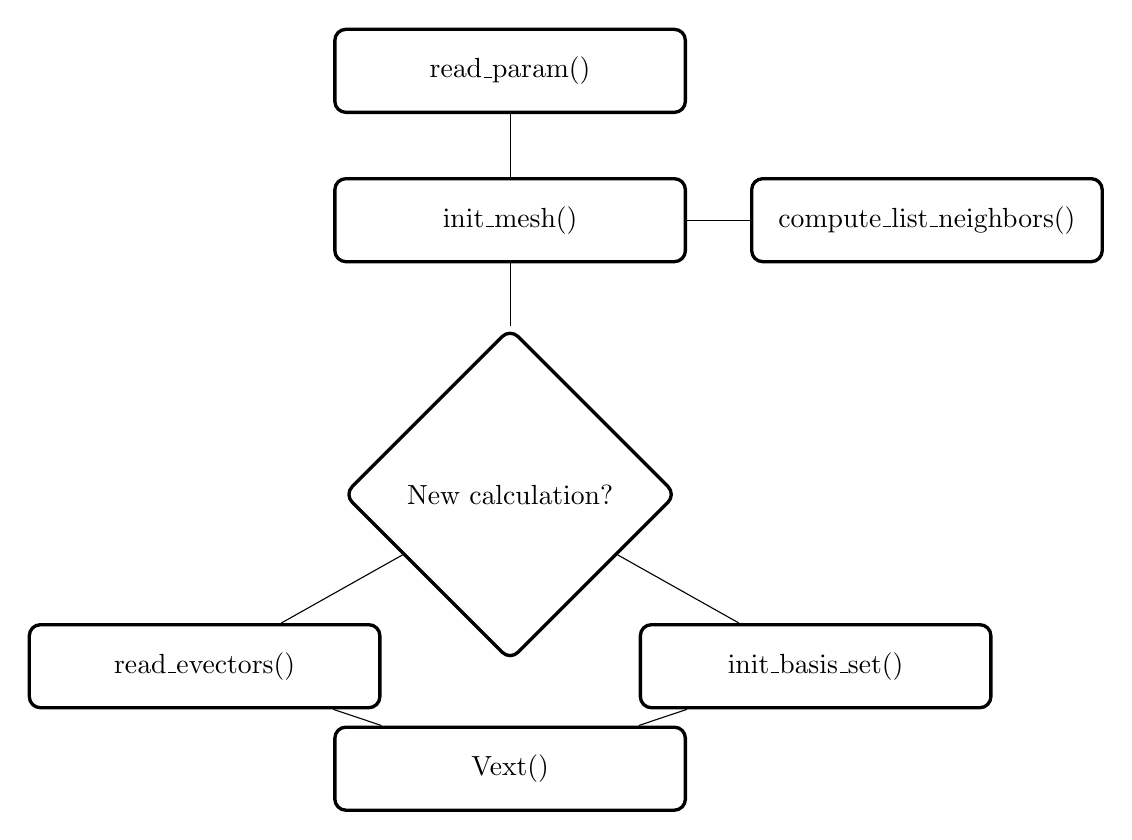
\begin{tikzpicture}[node distance=.8cm,start chain=going below,]
  \node[boite,join](read_param) {read\_param()};
  \node[boite,join](init_mesh) {init\_mesh()};
  \node[boite,](compute_list_neighbors)[right=of init_mesh] {compute\_list\_neighbors()};
  \draw[line] (init_mesh) edge (compute_list_neighbors);
  \node[boiteif](init_evec)[below=of init_mesh] {New calculation?};
  \draw[line] (init_mesh) edge (init_evec);
  \node[boite,](init_evec2)[below right= of init_evec] {init\_basis\_set()};
  \draw[line] (init_evec) edge (init_evec2);
  \node[boite,](init_evec3)[below left= of init_evec] {read\_evectors()};
  \draw[line] (init_evec) edge (init_evec3);
  \node[boite,](Vext)[below=of init_evec] {Vext()};
  \draw[line] (init_evec2) edge (Vext);
  \draw[line] (init_evec3) edge (Vext);
 \end{tikzpicture}

\begin{verbatim}
#! /bin/bash
####SBATCH -p public
#SBATCH -p grant -A g2018a7
###SBATCH -p grantgpu -Ag1018a7
#SBATCH -n 64 -tasks-per-node=64
#SBATCH -t 2:00:00                # Le job sera tue au bout de 1h
####SBATCH --mail-user=herve.bulou@ipcms.unistra.fr
#####SBATCH --mem=4096                # Quantite memoire demandee par noeud en Mo (unite obligatoire)


export OMP_NUM_THREADS=64
time ./Hbinitio.x

\end{verbatim}

\begin{verbatim}
module time_tracking
  implicit none
  type t_time
     real :: start,end,start_loc,end_loc
  end type t_time
contains
  ! -----------------------------------------------
  subroutine time_tracking_init(time_spent)
    implicit none
    type(t_time)::time_spent
    call cpu_time(time_spent%start)
    open(unit=1,file="dbg.dat",form='formatted',status='unknown')
    write(1,*)
    close(1)
  end subroutine time_tracking_init
  subroutine time_tracking_write(iloop,time_spent,text)
    integer :: iloop
    type(t_time)::time_spent
    character (len=*) :: text
    open(unit=1,file="dbg.dat",form='formatted',status='unknown',access='append')
    write(1,'(A50,I4,F12.6,F12.6,F12.6)') text,iloop,time_spent%end_loc,&
         time_spent%start_loc,time_spent%end_loc-time_spent%start_loc
    close(1)
  end subroutine time_tracking_write
end module time_tracking

  ! !!!!!!!!!!!!!!!!!!!!!!!!!!!!!!!!!!!!!!!!!!!!!!!!!!!!!!!!!!!!!!!!!!!!!!!!!!!!!!!!!!!!!!!!!!!!!!!!!!!!!!!
  ! !!!!!!!!!!!!!!!!!!!!!!!!!!!!!!!!!!!!!!!!!!!!!!!!!!!!!!!!!!!!!!!!!!!!!!!!!!!!!!!!!!!!!!!!!!!!!!!!!!!!!!!
  ! !!!!!!!!!!!!!!!!!!!!!!!!!!!!!!!!!!!!!!!!!!!!!!!!!!!!!!!!!!!!!!!!!!!!!!!!!!!!!!!!!!!!!!!!!!!!!!!!!!!!!!!
  ! !!!!!!!!!!!!!!!!!!!!!!!!!!!!!!!!!!!!!!!!!!!!!!!!!!!!!!!!!!!!!!!!!!!!!!!!!!!!!!!!!!!!!!!!!!!!!!!!!!!!!!!
  ! !!!!!!!!!!!!!!!!!!!!!!!!!!!!!!!!!!!!!!!!!!!!!!!!!!!!!!!!!!!!!!!!!!!!!!!!!!!!!!!!!!!!!!!!!!!!!!!!!!!!!!!
  ! !!!!!!!!!!!!!!!!!!!!!!!!!!!!!!!!!!!!!!!!!!!!!!!!!!!!!!!!!!!!!!!!!!!!!!!!!!!!!!!!!!!!!!!!!!!!!!!!!!!!!!!
program Hbinitio
  !$ use OMP_LIB
  use time_tracking
  implicit none
!  include 'mpif.h'
  type t_GramSchmidt
     integer :: nindep
     integer :: ndep ! number of linear dependencies discovered
  end type t_GramSchmidt
  type t_mesh
     integer :: Nx,Ny,Nz,N
     integer,allocatable :: list_neighbors(:,:),n_neighbors(:)
     double precision :: dx,dy,dz,dv
     double precision :: center(3)
  end type t_mesh
  type(t_mesh) :: mesh
  type t_cvg
     integer,allocatable:: list_cvg(:)
     integer :: ncvg
     double precision :: ETA
     integer :: nvec_to_cvg 
  end type t_cvg
  type(t_cvg) :: cvg
  type(t_time) :: time_spent
  type t_param
     logical::restart
     integer::ieof
     integer::loopmax
     integer::nvecini
     integer::nvecmax
     integer::Nx
     integer::nvec_to_cvg
     double precision :: ETA
     double precision::box_width
  end type t_param
  type(t_param)::param
  integer :: nvec
  integer,parameter :: seed = 86456
  double precision,allocatable :: V(:,:) ! wavefunctions
  double precision,allocatable :: Sprev(:),dS(:) ! eigenvalues
  double precision,allocatable :: pot_ext(:) ! external potential
  integer :: iloop
  character (len=1024) :: filecube
  character (len=1024)::line
  integer :: i

!  integer::ierr,my_id,num_procs
  ! !!!!!!!!!!!!!!!!!!!!!!!!!!!!!!!!!!!!!!!!!!!!!!

  call time_tracking_init(time_spent)

!  call mpi_init(ierr )
!  call MPI_COMM_RANK (MPI_COMM_WORLD, my_id, ierr)
!  call MPI_COMM_SIZE (MPI_COMM_WORLD, num_procs, ierr)

  call read_param(param)
  call init_mesh(mesh,param)  

!  nvecini=2
  nvec=param%nvecini
  allocate(V(mesh%N,nvec))
!  param%restart=.TRUE.
!  param%restart=.FALSE.
  if (.not.(param%restart))   then
     print *,"new calculation"
     call init_basis_set(V,nvec,seed,mesh)
  else
     print *,'restart an old calculation'
     call read_evectors(V,mesh,nvec)
  end if
  allocate(pot_ext(mesh%N))
  call Vext(mesh,pot_ext)
  
  open(unit=1,file="eigenvalues.dat",form='formatted',status='unknown'); write(1,*);  close(1)
  
  iloop=1
  cvg%ncvg=0
  cvg%nvec_to_cvg=param%nvec_to_cvg
  cvg%ETA=param%ETA
  allocate(Sprev(param%nvecini))
  allocate(dS(param%nvecini))
  Sprev(:)=0.0
  dS(:)=0.0
  do while((iloop.le.param%loopmax).and.(cvg%ncvg.lt.cvg%nvec_to_cvg))
     write(*,'(A)') 'Main > #######################################'     
     write(*,'(A,I4,A)') 'Main > ############ scf loop=',iloop,' ############'
     write(*,'(A)') 'Main > #######################################'     
     call davidson(nvec,V,mesh,param%nvecini,iloop,cvg,pot_ext,time_spent)
  end do
  call save_evectors(V,mesh,param%nvecini)
  do i=1,param%nvecini
     write(filecube,'(a,i0,a)') 'evec',i,'.cube'
     call norm(mesh,V(:,i))
     call save_cube(V(:,i),filecube,mesh)
  end do
  deallocate(V)
  deallocate(Sprev)
  deallocate(dS)
  deallocate(pot_ext)
  call free_mesh(mesh)
  call cpu_time(time_spent%end)
  if (cvg%ncvg.ge.cvg%nvec_to_cvg) print *,'Main > Job DONE !'
  print '("Main > Total Time = ",e16.6," seconds.")',time_spent%end-time_spent%start
!  call mpi_finalize(ierr)
  ! !!!!!!!!!!!!!!!!!!!!!!!!!!!!!!!!!!!!!!!!!!!!!!!!!!!!!!!!!!!!!!!!!!!!!!!!!!!!!!!!!!!!!!!!!!!!!!!!!!!!!!!
  ! !!!!!!!!!!!!!!!!!!!!!!!!!!!!!!!!!!!!!!!!!!!!!!!!!!!!!!!!!!!!!!!!!!!!!!!!!!!!!!!!!!!!!!!!!!!!!!!!!!!!!!!
  ! !!!!!!!!!!!!!!!!!!!!!!!!!!!!!!!!!!!!!!!!!!!!!!!!!!!!!!!!!!!!!!!!!!!!!!!!!!!!!!!!!!!!!!!!!!!!!!!!!!!!!!!
  ! !!!!!!!!!!!!!!!!!!!!!!!!!!!!!!!!!!!!!!!!!!!!!!!!!!!!!!!!!!!!!!!!!!!!!!!!!!!!!!!!!!!!!!!!!!!!!!!!!!!!!!!
  ! !!!!!!!!!!!!!!!!!!!!!!!!!!!!!!!!!!!!!!!!!!!!!!!!!!!!!!!!!!!!!!!!!!!!!!!!!!!!!!!!!!!!!!!!!!!!!!!!!!!!!!!
  ! !!!!!!!!!!!!!!!!!!!!!!!!!!!!!!!!!!!!!!!!!!!!!!!!!!!!!!!!!!!!!!!!!!!!!!!!!!!!!!!!!!!!!!!!!!!!!!!!!!!!!!!
contains
  ! --------------------------------------------------------------------------------------
  !
  !              read_param()
  !
  ! --------------------------------------------------------------------------------------
  subroutine read_param(param)
    implicit none
    type(t_param)::param
    integer::lline,eqidx
    double precision, parameter :: pi=3.1415927

    param%ieof=0
    param%loopmax=1000
    param%restart=.FALSE.
    param%nvecini=20
    param%nvecmax=41
    param%Nx=30
    param%nvec_to_cvg=20
    param%ETA=1.0e-3
    param%box_width=pi/sqrt(2.0)
    open(unit=1,file='inp',form='formatted')
    do while(.not.(is_iostat_end(param%ieof)))
       read(1,*,iostat=param%ieof) line
       lline=len_trim(line)
       eqidx=index(line,"=")
       print *,'###',eqidx,lline
       if(line(1:eqidx-1).eq."restart") then
          if(line(eqidx+1:lline).eq.'.TRUE.') then
             param%restart=.TRUE.
          else
             param%restart=.FALSE.
          end if
       end if
       if(line(1:eqidx-1).eq."loopmax") then
          read(line(eqidx+1:lline),*) param%loopmax
       end if
       if(line(1:eqidx-1).eq."nvecini") then
          read(line(eqidx+1:lline),*) param%nvecini
       end if
       if(line(1:eqidx-1).eq."nvecmax") then
          read(line(eqidx+1:lline),*) param%nvecmax
       end if
       if(line(1:eqidx-1).eq."Nx") then
          read(line(eqidx+1:lline),*) param%nx
       end if
       if(line(1:eqidx-1).eq."ETA") then
          read(line(eqidx+1:lline),*) param%ETA
       end if
       if(line(1:eqidx-1).eq."nvec_to_cvg") then
          read(line(eqidx+1:lline),*) param%nvec_to_cvg
       end if
       if(line(1:eqidx-1).eq."box_width") then
          read(line(eqidx+1:lline),*) param%box_width
       end if
       line=''
    end do
    close(1)


    print *,'#restart=',param%restart
    print *,'#loopmax=',param%loopmax
    print *,'#nvecini=',param%nvecini
    print *,'#nvecmax=',param%nvecmax
    print *,'#ETA=',param%ETA
    print *,'#nvec_to_cvg=',param%nvec_to_cvg
    print *,'#box_width=',param%box_width
    print *,'#Nx=',param%nx
    print *,'#dh=',param%box_width/(param%Nx+1)

  end subroutine read_param
  ! --------------------------------------------------------------------------------------
  !
  !              save_evectors()
  !
  ! --------------------------------------------------------------------------------------
  subroutine save_evectors(V,m,nvecini)
    implicit none
    type(t_mesh)::m
    double precision :: V(:,:)
    integer::nvecini,i,j
    open(unit=1,file="evectors.dat",form='formatted',status='unknown')
    do i=1,m%N
       write(1,*) (V(i,j),j=1,nvecini)
    end do
    close(1)
  end subroutine save_evectors
  ! --------------------------------------------------------------------------------------
  !
  !              read_evectors()
  !
  ! --------------------------------------------------------------------------------------
  subroutine read_evectors(V,m,nvecini)
    implicit none
    type(t_mesh)::m
    double precision :: V(:,:)
    integer::nvecini,i,j
    open(unit=1,file="evectors.dat",form='formatted',status='unknown')
    do i=1,m%N
       read(1,*) (V(i,j),j=1,nvecini)
    end do
    close(1)
  end subroutine read_evectors
  ! --------------------------------------------------------------------------------------
  !
  !              norm()
  !
  ! --------------------------------------------------------------------------------------
  subroutine  norm(m,evec) 
    implicit none
    double precision :: evec(:),normloc
    double precision, external :: ddot
    type(t_mesh)::m
    normloc=sqrt(m%dv*ddot(m%N,evec(:),1,evec(:),1))
    call dscal(m%N,normloc,evec(:),1)
  end subroutine norm
  ! --------------------------------------------------------------------------------------
  !
  !              Vext()
  !
  ! --------------------------------------------------------------------------------------
  subroutine Vext(m,pot_ext)
    implicit none
    type(t_mesh) :: m
    double precision :: pot_ext(:)
    double precision :: pts(3),rsqr
    
    character (len=1024) :: filename
    integer :: i,j,k,nn
    do k=1,m%Nz
       pts(3)=k*m%dz
       do i=1,m%Nx
          pts(1)=i*m%dx
          do j=1,m%Ny
             pts(2)=j*m%dy
             rsqr=(pts(1)-m%center(1))**2+(pts(2)-m%center(2))**2+(pts(3)-m%center(3))**2
             nn=j+(i-1)*m%Ny+(k-1)*m%Ny*m%Nx
             pot_ext(nn)=10*rsqr
          end do
       end do
    end do
    filename='pot_ext.cube'
    call save_cube(pot_ext,filename,m)
    !stop
  end subroutine Vext
  ! --------------------------------------------------------------------------------------
  !
  !              DAVIDSON()
  !
  ! --------------------------------------------------------------------------------------
  subroutine davidson(nvec,V,m,nvecini,iloop,cvg,pot_ext,time_spent)
    implicit none
    integer :: nvec,nvecini,iloop
    double precision,allocatable :: V(:,:),pot_ext(:)
    type(t_mesh) :: m
    type(t_cvg)::cvg
    type(t_time)::time_spent
    
    double precision,allocatable :: S(:) ! eigenvalues
    double precision,allocatable :: T(:,:) ! reduced matrix T
    double precision,allocatable :: VRitz(:,:) ! Ritz's vectors
    double precision,allocatable :: residual(:,:) ! residual
    double precision,allocatable :: delta(:,:) ! delta vectors
    double precision,allocatable :: Vnew(:,:) ! Vnew
    integer :: i
    integer :: ndelta
    integer :: newnvec
    type(t_GramSchmidt)::GS
    ! T (reduced matrix) computing
    allocate(T(nvec,nvec))
    call cpu_time(time_spent%start_loc)
    call compute_T(T,V,nvec,m,pot_ext)
    call cpu_time(time_spent%end_loc)
    call time_tracking_write(iloop,time_spent,'Davidson -> compute_T')
    
    ! Diagonatilzation of T
    allocate(S(nvec))

    call cpu_time(time_spent%start_loc)
    call diagonalization(S,T,nvec)
    call cpu_time(time_spent%end_loc)
    call time_tracking_write(iloop,time_spent,'Davidson -> Diagonalization')

    
    dS(:)=S(1:nvecini)-Sprev(:)
    Sprev(:)=S(1:nvecini)
    do i=1,nvecini
       write(*,'(A,I6,A,F12.6,A,E12.2,A)') 'Main > Eigenvalue(',i,'): ',S(i),'(',dS(i),')'
    end do
    !call cpu_time(inter)
    open(unit=1,file="eigenvalues.dat",form='formatted',status='unknown',access='append')
    write(1,*) iloop,S(1:nvecini)
    close(1)
    ! computation of the Ritz's vectors
    allocate(VRitz(m%N,nvec))

    call cpu_time(time_spent%start_loc)
    call Ritz(VRitz,V,T,nvec)
    call cpu_time(time_spent%end_loc)
    call time_tracking_write(iloop,time_spent,'Davidson -> Diagonalization')

    
    ! computation of residual
    allocate(residual(m%N,nvec))
    allocate(cvg%list_cvg(nvec))
    cvg%list_cvg(:)=0
    cvg%ncvg=0
    

    call cpu_time(time_spent%start_loc)
    call compute_residual(residual,VRitz,S,nvec,cvg,m,pot_ext)
    call cpu_time(time_spent%end_loc)
    call time_tracking_write(iloop,time_spent,'Davidson -> Residual')

    ! computation of delta
    allocate(delta(m%N,nvec))
    delta(:,:)=0.0
    !call cpu_time(inter)

    call cpu_time(time_spent%start_loc)
    call compute_delta(delta,residual,S,nvec,cvg,m,ndelta,pot_ext)
    call cpu_time(time_spent%end_loc)
    call time_tracking_write(iloop,time_spent,'Davidson -> Delta')

    
    deallocate(V)
    allocate(V(m%N,nvec+ndelta))
    V(:,1:nvec)=VRitz(:,:)
    print *,'ndelta=',ndelta
    print *,'nvec=',nvec
    V(:,nvec+1:nvec+ndelta)=delta(:,:ndelta)
    allocate(Vnew(m%N,nvec+ndelta))
    newnvec=nvec+ndelta
    GS%nindep=nvec
    !call cpu_time(inter)
    call GramSchmidt(Vnew,V,newnvec,m,GS)    
    ! call cpu_time(inter2);     call dbg(iloop,inter,inter2,'GS')
    
    print *,'Main > ',GS%ndep,newnvec
    
    deallocate(V)
    if(newnvec.le.param%nvecmax) then
       nvec=newnvec
    else
       print *,'Main > restart from nvecini'
       nvec=nvecini
    end if
    allocate(V(m%N,nvec))
    V(:,:)=Vnew(:,1:nvec)
    
    !call check_ortho(V,nvec,m)
    print *,'Main > New size of the basis ',nvec
    iloop=iloop+1
    deallocate(S)
    deallocate(T)
    deallocate(VRitz)
    deallocate(residual)
    deallocate(delta)
    deallocate(Vnew)
    deallocate(cvg%list_cvg)
  end subroutine davidson
  ! --------------------------------------------------------------------------------------
  !
  !              SAVE_CUBE()
  !
  ! --------------------------------------------------------------------------------------
  subroutine save_cube(data,filename,m)
    implicit none
    double precision :: data(:)
!    integer :: idxmin,idxmax
    type(t_mesh) :: m
    character (len=1024) :: filename
    
    character(len=*),parameter :: FMT1='(I5,3F12.6)'
    integer :: i,j,k,nn,ifield
    
    open(unit=1,file=filename,form='formatted',status='unknown')
    write(1,*) ' Cubefile created from Hbinitio.f90 calculation'
    write(1,*) ' H. Bulou, November 2018'
    write(1,FMT1) 1,0.0,0.0,0.0
    write(1,FMT1) m%Nx,m%dx,0.0,0.0
    write(1,FMT1) m%Ny,0.0,m%dy,0.0
    write(1,FMT1) m%Nz,0.0,0.0,m%dz
    write(1,'(I5,4F12.6)') 1,1.0,0.0,0.0,0.0
    do k=1,m%Nz
       ifield=0
       do i=1,m%Nx
          do j=1,m%Ny
             nn=j+(i-1)*m%Ny+(k-1)*m%Ny*m%Nx               
             write(1,'(E13.5)',advance='no') data(nn)
             ifield=ifield+1
             if (mod(ifield,6).eq.0) then
                ifield=0
                write(1,*)
             end if
          end do
       end do
       write(1,*)
    end do
    close(1)
  end subroutine save_cube

  ! --------------------------------------------------------------------------------------
  !
  !              COMPUTE_DELTA()
  !
  ! --------------------------------------------------------------------------------------
  subroutine compute_delta(delta,r,lambda,nvec,cvg,m,ndelta,pot_ext)
    ! INPUT: the residual |r>, the Ritz's vectors |VRitz>, the eigenvalues lambda
    ! OUTPUT : the correction |delta> to improve the  Ritz's vectors so that to
    !          minimize the residual
    implicit none
    type(t_mesh)::m
    double precision :: lambda(:),r(:,:),delta(:,:),pot_ext(:)
    integer :: nvec,ndelta
    type(t_cvg)::cvg
    
    double precision, external :: ddot
    double precision, parameter::alpha=1.0,beta=0.0
    double precision, allocatable :: normloc
!    double precision, allocatable :: Dinv(:,:)
    integer :: i,j
    double precision :: deltasqr

    deltasqr=m%dx**2
    print *,'Delta > ---------------------'
    print *,'Delta > --- compute_delta ---'
    print *,'Delta > ---------------------'
    !delta(:,:)=0.0
   ! allocate(Dinv(m%N,m%N))
  !  Dinv(:,:)=0.0
    ndelta=0
    do i=1,nvec
       if(cvg%list_cvg(i).eq.0) then
          ndelta=ndelta+1
          do j=1,m%N
             delta(j,ndelta)=r(j,ndelta)/((3.0/deltasqr+pot_ext(j))-lambda(i))
!             Dinv(j,j)=1.0/((3.0/deltasqr+pot_ext(j))-lambda(i))
          end do
          ! see Victor Eijkhout in "Introduction to scientific and technical computing" edited by Willmore et al
          ! Chap 15 Libraries for Linear Algebra
          ! to get a comprehensive way to use dgemv
 !         call dgemv('N',m%N,m%N,alpha,Dinv,m%N,r(:,ndelta),1,beta,delta(:,ndelta),1)
          !norm=sqrt(ddot(m%N,delta(:,i),1,delta(:,i),1))
          !write(*, '(A10,I4,A2,E12.6)',advance='no') ' Delta > delta(',i,')=',norm
          !delta(:,ndelta)=delta(:,ndelta)+VRitz(:,ndelta)
          normloc=1.0/sqrt(ddot(m%N,delta(:,ndelta),1,delta(:,ndelta),1))
          call dscal(m%N,normloc,delta(:,ndelta),1)
       end if
    end do
    !deallocate(Dinv)
    print *,'Delta > ',ndelta,' new vector(s)'
  end subroutine compute_delta
    
  
  ! --------------------------------------------------------------------------------------
  !
  !              COMPUTE_RESIDUAL()
  !
  ! --------------------------------------------------------------------------------------
  subroutine compute_residual(r,VRitz,S,nvec,cvg,m,pot_ext)
    implicit none
    type(t_mesh)::m
    integer :: nvec
    double precision :: r(:,:),VRitz(:,:),S(:),pot_ext(:)
    type(t_cvg) :: cvg

    integer :: i,j,k
    double precision :: normloc
    double precision, external :: ddot        
    double precision :: deltasqr

    print *,'Residual > ------------------------'
    print *,'Residual > --- compute residual ---'
    print *,'Residual > ------------------------'
    deltasqr=m%dx**2
    r(:,:)=0.0
    cvg%ncvg=0
    do j=1,nvec
       do i=1,m%N
          r(i,j)=(3.0/deltasqr+pot_ext(i))*VRitz(i,j)
          do k=1,m%n_neighbors(i)
             r(i,j)=r(i,j)-0.5*VRitz(m%list_neighbors(i,k),j)/deltasqr
          end do
          r(i,j)=r(i,j)-S(j)*VRitz(i,j)
       end do
       normloc=ddot(m%N,r(:,j),1,r(:,j),1)
       write(*,'(A,I4,A,E12.4,A,E12.4)',advance='no') 'Residual > r(',j,')= ',normloc,'/',cvg%ETA
       if (normloc.lt.cvg%ETA) then
          cvg%ncvg=cvg%ncvg+1
          cvg%list_cvg(j)=1
          write(*,*) '--> converged'
       else
          write(*,*)
       end if
       
    end do
  end subroutine compute_residual
  
  ! --------------------------------------------------------------------------------------
  !
  !              RITZ()
  !
  ! --------------------------------------------------------------------------------------
  subroutine Ritz(Vout,Vin,y,nvec)
    implicit none
    double precision :: Vin(:,:),Vout(:,:),y(:,:)
    integer :: nvec

    integer :: i,j
    print *,'Ritz > --------------'
    print *,'Ritz > --- Ritz() ---'
    print *,'Ritz > --------------'
    do i=1,nvec
       Vout(:,i)=y(1,i)*Vin(:,1)
       do j=2,nvec
          Vout(:,i)=Vout(:,i)+y(j,i)*Vin(:,j)
       end do
    end do
  end subroutine Ritz
  
  
  ! --------------------------------------------------------------------------------------
  !
  !              DIAGONALIZATION()
  !
  ! --------------------------------------------------------------------------------------
  subroutine diagonalization(S,H,N)
    implicit none
    integer :: N
    double precision :: H(:,:),S(:)

    integer :: lwork,info
    integer :: lwmax
    double precision,allocatable::work(:)
    parameter(lwmax=100000)
    allocate(work(lwmax))
    lwork=-1
    call  dsyev('vectors','Upper',N,H,N,S,work,lwork,info)
    lwork=min(lwmax,int(work(1)))
    if (lwork.ge.lwmax) then
       write(*,*) 'Diagonalization > WARNING info = ',info
       write(*,*) 'Diagonalization > WARNING lwork=',lwork
       write(*,*) 'Diagonalization > WARNING size of work(1)',int(work(1))
       stop
    end if
    call  dsyev('vectors','Upper',N,H,N,S,work,lwork,info)
    if(info.gt.0) then
       write(*,*) "Diagonalization > WARNING The algorithm computing failed"
       stop
    end if
    deallocate(work)
  end subroutine diagonalization
  
  
  ! --------------------------------------------------------------------------------------
  !
  !              COMPUTE_T()
  !
  ! --------------------------------------------------------------------------------------
  subroutine compute_T(T,V,nvec,m,pot_ext)
    implicit none
    double precision,allocatable :: V(:,:),T(:,:),pot_ext(:)
    integer :: nvec
    type(t_mesh)::m
    
    integer :: i,j,k,l
    double precision :: deltasqr,acc
    double precision, parameter::alpha=0.0
!    double precision::beta
    
    deltasqr=m%dx**2
    !$OMP PARALLEL private(acc) 
    !$OMP DO 
    do j=1,nvec
       do i=1,nvec ! Tij
          T(i,j)=0.0
          do k=1,m%N
             acc=(3.0/deltasqr+pot_ext(k))*V(k,j) ! the potential will be added here
             do l=1,m%n_neighbors(k)
                acc=acc-0.5*V(m%list_neighbors(k,l),j)/deltasqr
!                print *, omp_get_thread_num(),i,j,k,l
             end do
             T(i,j)=T(i,j)+V(k,i)*acc
!             print *,' -> ',omp_get_thread_num(),i,j,T(i,j)
          end do
!          print *,omp_get_thread_num(),i,j,T(i,j)
       end do
    end do
    !$OMP END DO
    !$OMP END PARALLEL
!    stop
  end subroutine compute_T
  
  
  ! --------------------------------------------------------------------------------------
  !
  !              INIT_BASIS_SET()
  !
  ! --------------------------------------------------------------------------------------
  subroutine init_basis_set(V,nvec,seed,m)
    implicit none
    integer :: nvec,seed
    double precision,allocatable :: V(:,:)
    type(t_mesh)::m

    double precision, external :: ddot
    double precision ::normloc
    integer :: i,j
    double precision,allocatable :: Vdump(:,:)
    type(t_GramSchmidt) :: GS
    
    allocate(Vdump(m%N,nvec))
    call srand(seed)
    do i=1,nvec
       do j=1,m%N
          Vdump(j,i)=rand()
       end do
    end do
    do i=1,nvec
       normloc=ddot(m%N,Vdump(:,i),1,Vdump(:,i),1)
       normloc=1.0/sqrt(normloc)
       call dscal(m%N,normloc,Vdump(:,i),1)
    end do
    GS%nindep=1
    call GramSchmidt(V,Vdump,nvec,m,GS)

    deallocate(Vdump)
  end subroutine init_basis_set
  ! -----------------------------------------------
  ! Ref.: D. G. Clayton "Gram-Schmidt Orthogonalization", J. Roy. Stat. Soc. C 20, 335 (1971)
  subroutine GramSchmidt(Vout,Vin,nvec,m,GS)
    implicit none
    integer ::  nvec
    double precision,allocatable :: Vin(:,:),Vout(:,:)
    type(t_mesh)::m
    type(t_GramSchmidt) :: GS
    
    integer :: i,k,i0
    double precision, parameter :: ETA=1.0e-6
    double precision,allocatable :: a(:)
    double precision :: normloc
    double precision, external :: ddot

    allocate(a(nvec))
    print *,'GS> ----------------------'
    print *,"GS> Gram-Schmidt algorithm"
    print *,'GS> ----------------------'
    print *,'GS> ',nvec,' vectors to orthogonalize'
    print *,'GS> ',GS%nindep,' vectors are already orthogonalized'
    Vout(:,1:GS%nindep)=Vin(:,1:GS%nindep)
    GS%ndep=0 
    i0=GS%nindep
    do i=i0+1,nvec
       Vout(:,GS%nindep+1)=Vin(:,i)
       do k=1,GS%nindep
          ! We compute the projection of Vini(:,i) on V(:,1-nindep)
          a(k)=ddot(m%N,Vout(:,k),1,Vin(:,i),1)
          !print *,'GS > ',i,k,a(k)
          ! then we remove V(:,k) from V(:,nindep+1)
          call daxpy(m%N,-a(k),Vout(:,k),1,Vout(:,GS%nindep+1),1)
       end do
       ! now wre compute the norm of V(:,nindep+1)
       normloc=sqrt(ddot(m%N,Vout(:,GS%nindep+1),1,Vout(:,GS%nindep+1),1))
       !print *,'GS > norm(',i,')=',norm
       if (normloc.le.ETA) then
          GS%ndep=GS%ndep+1 ! V(:,nindep+1) is not linearly inependent
       else
          normloc=1.0/normloc
          call dscal(m%N,normloc,Vout(:,GS%nindep+1),1)
          !              do k=2,icur
          !                 print *,'<U',k-1,'|U',i,'>=',ddot(N,V(:,k-1),1,V(:,icur),1)
          !              end do
          GS%nindep=GS%nindep+1
       end if
    end do
    print *,'GS> ',GS%ndep,' vectors linearly dependant'
    print *,'GS> ',GS%nindep,' vectors linearly independant'
    print *,'GS> Size of the basis from ',nvec,' to ',GS%nindep
    !call check_ortho(Vout,nvec,m)
    !stop
    nvec=GS%nindep
    deallocate(a)
  end subroutine GramSchmidt
  ! -----------------------------------------------
  subroutine check_ortho(P,nvec,m)
    implicit none
    integer :: nvec
    double precision :: P(:,:)
    type(t_mesh)::m

    double precision, parameter :: ETA=1.0e-6
    integer :: i,j,nfail
    double precision :: pscal
    double precision, external :: ddot
    nfail=-nvec
    print *,"--- check_ortho() ---"      
    do i=1,nvec
       do j=1,nvec
          pscal=ddot(m%N,P(:,i),1,P(:,j),1)
          write(*,'(F10.2)',advance='no') pscal
          if (pscal.gt.ETA) nfail=nfail+1
       end do
       write(*,*)
    end do
    if (nfail.gt.0) then
       print *,nfail,' fail(s)'
       stop
    end if
  end subroutine check_ortho
  

  ! -----------------------------------------------
  subroutine init_mesh(m,param)
    implicit none
    type(t_mesh)::m
    type(t_param)::param
    double precision:: Lwidth 

    Lwidth=param%box_width
    m%Nx=param%Nx
!    m%Nx=5
    m%Ny=m%Nx
    m%Nz=m%Nx
    m%N=m%Nx*m%Ny*m%Nz

    m%dx=Lwidth/(m%Nx+1)
    m%dy=Lwidth/(m%Ny+1)
    m%dz=Lwidth/(m%Nz+1)
    m%dv=m%dx*m%dy*m%dz
    !m%dv=1.0

    m%center(1)=Lwidth/2
    m%center(2)=Lwidth/2
    m%center(3)=Lwidth/2
    
    allocate(m%n_neighbors(m%N))
    allocate(m%list_neighbors(m%N,6)) !
    m%list_neighbors(:,:)=0
    m%n_neighbors(:)=0
    call compute_list_neighbors(m)
  end subroutine init_mesh
  ! -----------------------------------------------
  subroutine free_mesh(m)
    implicit none
    type(t_mesh) :: m
    deallocate(m%n_neighbors)
    deallocate(m%list_neighbors) !
  end subroutine free_mesh
  ! -----------------------------------------------
  subroutine compute_list_neighbors(m)
    implicit none
    type(t_mesh) :: m
    integer::i,j,k,nn
    !integer,allocatable::n_neighbors(:),list_neighbors(:,:)
    
    do k=1,m%Nz
       do i=1,m%Nx
          do j=1,m%Ny
             nn=j+(i-1)*m%Ny+(k-1)*m%Ny*m%Nx
             if (k>1) then 
                m%n_neighbors(nn)=m%n_neighbors(nn)+1
                m%list_neighbors(nn,m%n_neighbors(nn))=nn-m%Nx*m%Ny
             end if
             if (k<m%Nz) then 
                m%n_neighbors(nn)=m%n_neighbors(nn)+1
                m%list_neighbors(nn,m%n_neighbors(nn))=nn+m%Nx*m%Ny
             end if
             if (i>1) then 
                m%n_neighbors(nn)=m%n_neighbors(nn)+1
                m%list_neighbors(nn,m%n_neighbors(nn))=nn-m%Ny
             end if
             if (i<m%Nx) then 
                m%n_neighbors(nn)=m%n_neighbors(nn)+1
                m%list_neighbors(nn,m%n_neighbors(nn))=nn+m%Ny
             end if
             if (j>1) then 
                m%n_neighbors(nn)=m%n_neighbors(nn)+1
                m%list_neighbors(nn,m%n_neighbors(nn))=nn-1
             end if
             if (j<m%Ny) then 
                m%n_neighbors(nn)=m%n_neighbors(nn)+1
                m%list_neighbors(nn,m%n_neighbors(nn))=nn+1
             end if
          end do
       end do
    end do

  end subroutine compute_list_neighbors
  
  
end program Hbinitio
\end{verbatim}
\end{document}
